% GENERATED, edit the French unit or the translation table
\mxunit{seconde-s14}{Probability: conditioning and weighted trees}\mxsubtitle{26 April--24 May 2027}
\section{Sample space, outcomes and events}
\begin{keypoint}[Vocabulary]
A random experiment has several possible results, without it being known in advance which will occur. An outcome is a possible result; the sample space $\Omega$ is the set of them. An event is a subset of $\Omega$; an elementary event contains a single outcome.
The impossible event is $\varnothing$; the certain event is $\Omega$.
\end{keypoint}
\begin{keypoint}[Operations on events]
$\overline A$ is the complementary event of $A$. $A\cap B$ means ``$A$ and $B$''; $A\cup B$, ``$A$ or $B$'', possibly both. Two events are mutually exclusive if $A\cap B=\varnothing$; otherwise, they are compatible.
\end{keypoint}
\begin{example}A six-sided die is rolled. Write $\Omega$, $A$: ``get an even number'', $B$: ``get $4$'', then $\overline A$, $A\cap B$ and $A\cup B$. Are $A,B$ compatible?\end{example}
\mxanswerspace[4]{$\Omega=\{1;2;3;4;5;6\}$, $A=\{2;4;6\}$, $B=\{4\}$, $\overline A=\{1;3;5\}$, $A\cap B=\{4\}$, $A\cup B=A$. The events are compatible because they share the outcome $4$.}
\begin{example}With $A=\{a;b;c;d;e\}$ and $B=\{b;e;f;g;h\}$, give the intersection and the union. Can $\overline A$ be determined without specifying the sample space?\end{example}
\mxanswerspace[3.2]{$A\cap B=\{b;e\}$ and $A\cup B=\{a;b;c;d;e;f;g;h\}$. The complement depends on the sample space; it cannot be determined without this information.}

\mxsection{Probability model and equally likely outcomes}
\begin{keypoint}[Probability on a finite sample space]
To each outcome, a model assigns a probability that is positive or zero; the sum is $1$. The probability of an event is the sum of the probabilities of its outcomes. We have
\[P(\Omega)=1,\quad P(\varnothing)=0,\quad P(\overline A)=1-P(A).\]
With equally likely outcomes, all outcomes have the same probability and
\[P(A)=\frac{\Card(A)}{\Card(\Omega)}.\]
Equal likelihood is an assumption of the model, not a consequence of the list of outcomes alone.
\end{keypoint}
\begin{example}Assume the die is fair. For $A=$ ``even'' and $C=$ ``greater than or equal to $5$'', calculate $P(A)$, $P(C)$, $P(A\cap C)$ and $P(A\cup C)$.\end{example}
\mxanswerspace[4]{$P(A)=3/6=1/2$, $P(C)=2/6=1/3$, $A\cap C=\{6\}$ so $P(A\cap C)=1/6$. $A\cup C=\{2;4;5;6\}$, so $P(A\cup C)=4/6=2/3$. The outcome $6$ must not be counted twice.}
\begin{example}A drawing pin can land point up or point down. Can we deduce that each outcome has probability $1/2$? How can a model be proposed?\end{example}
\mxanswerspace[4]{No: two outcomes are not enough to impose equal likelihood. One can repeat the throws under comparable conditions and use the observed frequencies to propose a model, bearing in mind fluctuations and the characteristics of the object.}
\begin{teachernote}Reactivate the link between observed frequency and postulated probability. An experimental result does not prove exact equal likelihood.\end{teachernote}

\mxsection{Conditional probability from a table}
\begin{keypoint}[Definition]
For $P(A)>0$, the probability of $B$ given $A$ is
\[P_A(B)=\frac{P(A\cap B)}{P(A)},\qquad P(A\cap B)=P(A)P_A(B).\]
For an equally likely draw within a finite population:
\[P_A(B)=\frac{\Card(A\cap B)}{\Card(A)}.\]
We also write $P(B\mid A)$. $P_A(B)$ and $P_B(A)$ are generally not equal.
\end{keypoint}
\begin{example}A student is drawn uniformly from the class of $32$ students studied earlier. $G$: ``boy'', $N$: ``takes CS''.\end{example}
\begin{center}\mxarraystretch{1.5}\begin{tabular}{c|rr|r}
&$G$&$\overline G$&Total\\\hline
$N$&12&9&21\\$\overline N$&6&5&11\\\hline Total&18&14&32
\end{tabular}\end{center}
Calculate $P(G)$, $P(N)$, $P(G\cap N)$, $P_N(G)$ and $P_G(N)$.
\mxanswerspace[5]{$P(G)=18/32=9/16$, $P(N)=21/32$, $P(G\cap N)=12/32=3/8$.
$P_N(G)=12/21=4/7$, whereas $P_G(N)=12/18=2/3$.
By the formula: $P_N(G)=(12/32)/(21/32)=12/21$. Given that the student takes CS, the reference population is reduced to the $21$ students concerned.}
\begin{pitfall}Conditioning requires the known event to have nonzero probability; we do not divide by zero.\end{pitfall}

\mxsection{Weighted trees and the probability of a path}
\begin{keypoint}[Rules]
At each node, the sum of the probabilities of the outgoing branches is $1$. A second-level branch carries a conditional probability. A path represents an intersection of events; its probability is the product of the probabilities written along that path.
\end{keypoint}
\begin{center}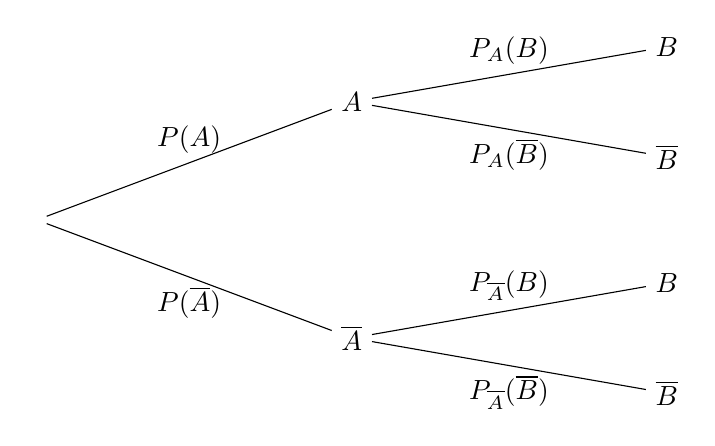
\begin{tikzpicture}[grow=right,level 1/.style={level distance=4cm,sibling distance=3cm},level 2/.style={level distance=4cm,sibling distance=1.4cm},edge from parent/.style={draw},every node/.style={font=\normalsize}]
\node{} child{node{$\overline A$} child{node{$\overline B$} edge from parent node[below]{$P_{\overline A}(\overline B)$}} child{node{$B$} edge from parent node[above]{$P_{\overline A}(B)$}} edge from parent node[below]{$P(\overline A)$}} child{node{$A$} child{node{$\overline B$} edge from parent node[below]{$P_A(\overline B)$}} child{node{$B$} edge from parent node[above]{$P_A(B)$}} edge from parent node[above]{$P(A)$}};
\end{tikzpicture}\end{center}
\begin{example}We know $P(A)=0.6$, $P_A(B)=0.7$ and $P_{\overline A}(\overline B)=0.9$. Complete the other branches and calculate the probabilities of the four paths.\end{example}
\mxanswerspace[5]{$P(\overline A)=0.4$, $P_A(\overline B)=0.3$, $P_{\overline A}(B)=0.1$.
\[P(A\cap B)=0.6\times0.7=0.42,\quad P(A\cap\overline B)=0.18,\]
\[P(\overline A\cap B)=0.04,\qquad P(\overline A\cap\overline B)=0.36.\]
The sum of the four probabilities is $1$, which checks the consistency of the model.}
\begin{example}Justify the multiplication along the path $A$ then $B$ from the definition of $P_A(B)$.\end{example}
\mxanswerspace[2.4]{Since $P_A(B)=P(A\cap B)/P(A)$ and $P(A)>0$, multiplying by $P(A)$ gives $P(A)P_A(B)=P(A\cap B)$.}

\mxsection{From a table to a tree}
\begin{example}For the class of $32$ students, construct a tree starting with CS / no CS, then boy / girl. Then construct the tree in the reverse order. Check, in both trees, the probability of choosing a girl who takes CS.\end{example}
\mxanswerspace[7]{First tree: initial branches $P(N)=21/32$, $P(\overline N)=11/32$. After $N$: $P_N(G)=12/21=4/7$, $P_N(\overline G)=9/21=3/7$. After $\overline N$: $6/11$ and $5/11$.
Second tree: initial branches $P(G)=18/32=9/16$, $P(\overline G)=14/32=7/16$. After $G$: $P_G(N)=12/18=2/3$, then $1/3$. After $\overline G$: $P_{\overline G}(N)=9/14$, then $5/14$.
The required path is worth $(21/32)(9/21)=9/32$ in the first tree and $(14/32)(9/14)=9/32$ in the second. Changing the order preserves the probabilities of the intersections but changes the probabilities of the branches.}
\begin{example}An urn contains $3$ red balls and $2$ blue balls. Two balls are drawn in succession \textbf{without replacement}. Construct the tree of colours and calculate the probability of drawing two red balls.\end{example}
\mxanswerspace[5]{First level: $R$ with $3/5$, $B$ with $2/5$. After $R$, $2$ red and $2$ blue remain: branches $1/2,1/2$. After $B$, $3$ red and $1$ blue remain: branches $3/4,1/4$. So $P(R_1\cap R_2)=(3/5)(1/2)=3/10$. Using $3/5$ on the second red branch would ignore the absence of replacement.}

\mxsection{Inverting conditioning and false positives}
\begin{example}[Fictional component check]A batch contains $10000$ components, of which $100$ are defective. A test is positive for $99$ of the defective components and for $495$ of the non-defective components. A component is chosen uniformly. $D$: ``defective''; $T$: ``test positive''.
\begin{enumerate}\item Complete the two-way table of test / true state.\item Calculate $P_D(T)$ and $P_T(D)$.\item Give the number of false positives and false negatives.\item Calculate the sensitivity $P_D(T)$ and the specificity $P_{\overline D}(\overline T)$.\end{enumerate}\end{example}
\mxanswerspace[7]{
\begin{center}\mxarraystretch{1.5}\begin{tabular}{c|rr|r}&$D$&$\overline D$&Total\\\hline $T$&99&495&594\\$\overline T$&1&9405&9406\\\hline Total&100&9900&10000\end{tabular}\end{center}
$P_D(T)=99/100=99\,\%$. On the other hand $P_T(D)=99/594=1/6\approx16.67\,\%$. A positive test therefore does not imply here a $99\,\%$ probability of defect.
The $495$ false positives are the sound components that tested positive; the false negative is the defective component that tested negative. The sensitivity is $99\,\%$; the specificity $9405/9900=95\,\%$.
The low initial proportion of defective components explains why false positives outnumber true positives despite the good sensitivity.}
\begin{keypoint}[Reading a test result]
``Positive among the defective'' and ``defective among the positives'' correspond to two different conditionings. Always name the reference group before the calculation.
\end{keypoint}
\begin{teachernote}The numbers are fictional. The table allows studying the inversion without requiring a general total-probability formula: this is not an expectation of the 2026 Seconde programme.\end{teachernote}

\mxsection{Simulation and the law of large numbers}
\begin{keypoint}[Popularised version]
When an experiment is repeated a large number of times in the same model with independent repetitions, the observed frequency of an event is, barring exceptions, close to its probability. It fluctuates: it does not necessarily get closer with each new trial.
\end{keypoint}
\begin{lstlisting}
from random import Random

def frequences_six(n, graine=1):
    # n entier >= 1 ; modele de lancers independants
    rng = Random(graine)
    succes = 0
    frequences = []
    for k in range(1, n+1):
        if rng.randint(1, 6) == 6:
            succes = succes+1
        frequences.append(succes/k)
    return frequences
\end{lstlisting}
\begin{example}Plot the frequencies for $n=1000$, with several seeds. Compare with $1/6$. Why fix the seed? Can we require the final frequency to be exactly $1/6$?\end{example}
\mxanswerspace[4]{The plots depend on the seed and fluctuate around $1/6$. Fixing the seed makes the simulation reproducible. With $1000$ throws, a final frequency of exactly $1/6$ is even impossible, because $1000/6$ is not an integer. A nearby frequency is consistent with the model, but is not a proof of it.}
\begin{example}Modify the program to track the frequency of the event ``even result''. Which reference probability should be used?\end{example}
\mxanswerspace[3.2]{Replace the test with \texttt{rng.randint(1, 6) \% 2 == 0}. The reference probability is $3/6=1/2$. Each trial must make a single draw; do not call the generator several times to test the same result.}
